\documentclass[a4paper]{article}
\usepackage{geometry}
\usepackage[utf8]{inputenc}
\usepackage[T1]{fontenc}
\usepackage[bookmarks,hidelinks]{hyperref}
\usepackage[french]{babel}
\usepackage{pdflscape}
\usepackage{graphicx}
\usepackage{afterpage}
\usepackage{listings}

\title{Rapport du projet de Technologies Objets}
\author{Maxime Arthaud \and Korantin Auguste \and Martin Carton}
\date{11 juin 2013}

\begin{document}
\maketitle 
\tableofcontents
\newpage

\section{Introduction}
  Ce projet consiste en la création d'une interface utilisateur permettant de
  gérer une scène 3D et à la réalisation d'un moteur de rendu par lancé de
  rayons.

  Comme expliqué dans le rapport d'analyse, nous avons décidé de nous découper
  le travail, de façon à ce qu'une personne fasse l'interface graphique,
  une autre le parseur de fichier et l'écriture d'images au format PPM, et une
  autre travaille particulièrement sur le cœur du raytracer.

\section{Architecture}
  Le projet est donc constitué de deux programmes distincts:
  \begin{description}
      \item[L'interface graphique] Qui devra permettre de créer simplement des
        fichiers représentant des scènes, à passer à notre raytracer.
      \item[Le raytracer] Qui, à partir d'un fichier représentant une scène,
        devra générer un rendu, dans le format d'image de notre choix.
  \end{description}

  \subsection{Écriture d'images PPM}
    Pour écrire les images PPM, nous avons écrit un plugin Java qui permet
    d'enregistrer ce format auprès de \verb+javax.image.ImageIO+ qui propose une
    interface commune pour enregistrer des images dans différents formats. Ainsi
    notre programme peut générer des images au format PPM, mais aussi par
    exemple en PNG. Le choix de ce format est déterminé par l'extension du
    fichier de sortie fournie au programme.

    Ce plugin consiste en deux classes \verb+imageio.PPMImageWriterSpi+ et
    \verb+imageio.PPMImageWriterSpi+. La première permet d'indiquer à Java les
    capacité de notre plugin. La deuxième permet d'écrire une image sur un flux
    de sortie quelconque.

  \subsection{Format de fichier}
    Nous avons décidé de mettre à disposition un format de fichier dans lequel
    on peut décrire une scène afin de pouvoir enregistrer celles-ci, ou de la
    générer automatiquement.

    Le format de fichier ressemble à ceci:
    \begin{lstlisting}
#exemple de scene :
Camera(eye=(0, 0, 0), origin=(-0.5, -0.5, 1), abscissa=(1, 0, 0), \
ordinate=(0, 1, 0), widthPixel=1000, heightPixel=1000)
AmbientLights(0.2, 0.2, 0.2)
Light(pos=(5, 0, 0), intensity=(0.5, 0.5, 0.5))
Sphere(center=(0, 5, 20), radius=3.14, k_diffuse=(0.6,0.3,0.6))
Plan(p1=(0,0,30), p2=(1, 0, 30), p3=(0, 1, 30))
    \end{lstlisting}

    Il y a un élément par ligne et seule la ligne décrivant la caméra est
    obligatoire. La casse et l'espacement sont ignorés. La plupart des
    propriétés ont une valeur par défaut afin d'éviter de surcharger le
    fichier et de permettre de l'écrire à la main. Des commentaires de fin de
    ligne commençant par «~\verb+//+~» peuvent être insérés.

    Les éléments suivants peuvent être ajoutés:
    \begin{description}
      \item[Camera] décrit la caméra de la scène: elle doit posséder les
        propriétés suivantes:
        \begin{description}
          \item[eye] un point décrivant la position de l'œil;
          \item[origin] un point décrivant l'origine du rectangle de l'écran;
          \item[abscissa et ordinate] les vecteurs qui avec \textit{origin}
            définissent l'écran;
          \item[widthPixel et heightPixem] deux entiers donnant la taille de
            l'image à générer. 
        \end{description}
      \item[AmbientLights] donne les trois composantes primaire de la lumière
        ambiante.
      \item[Light] décrit une source de lumière, elle doit avoir les propriétés
        suivantes:
        \begin{description}
          \item[pos] la position de cette source;
          \item[intensity] l'intensité lumineuse de chaque couleur primaire.
        \end{description}
      \item[Sphere] décrit une sphère, doit avoir les propriétés suivantes:
        \begin{description}
          \item[center] un point représentant le centre de la sphère;
          \item[radius] un flottant représentant le rayon de la sphère.
        \end{description}
      \item[Plane] décrit un plan, doit avoir trois points nommés \textit{P1},
        \textit{P2} et \textit{P3}.
      \item[Triangle] décrit un triangle, doit avoir trois points nommés
        \textit{P1}, \textit{P2} et \textit{P3}.
      \item[Cube] décrit un cube, doit avoir quatre points nommés
        \textit{P1}, \textit{P2}, \textit{P3} et \textit{P4} répartis comme
        ceci: \begin{lstlisting}
   p2------+
  /|      /|
 / |     / |
p1------p3 |
|  +----|--+
| /     | /
|/      |/
p4------+
        \end{lstlisting}
    \end{description}

    \bigskip
    Les objets \textit{Sphere}, \textit{Plane}, \textit{Triangle} et
    \textit{Cube} peuvent en plus avoir les propriétés suivantes:
    \begin{description}
      \item[brightness] flottant, par défaut à 30;
      \item[k\_specular] flottant, par défaut à 1;
      \item[k\_diffuse] vecteur, par défaut à \textit{(1, 1, 1)};
      \item[k\_reflection] flottant, par défaut à 1;
      \item[k\_refraction] vecteur, par défaut à \textit{(0, 0, 0)};
      \item[refractive\_index] flottant, par défaut à 1.
    \end{description}

    \bigskip
    Un objet de type \verb+Scene+ est construit à partir d'un tel fichier à
    l'aide la méthode statique \verb+raytracer.FileReader.read+.

  \subsection{Interface graphique}
    Maxime ?

    \begin{figure}[p]
      \centerline{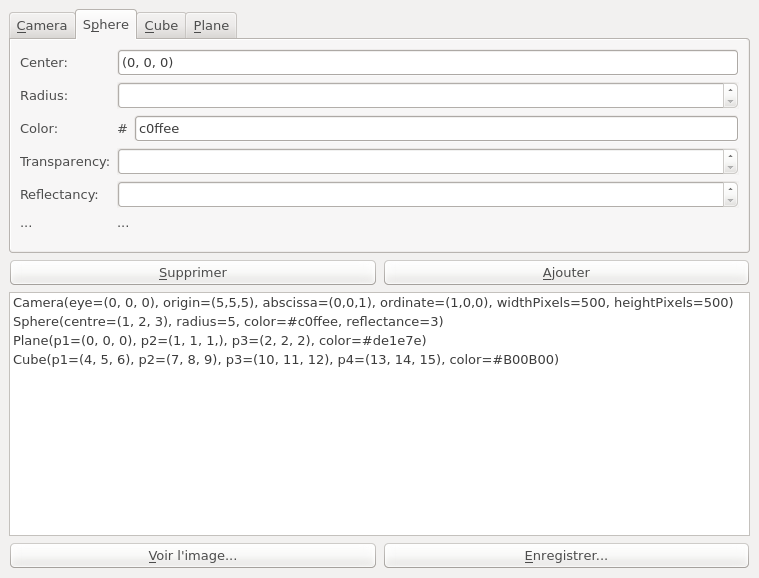
\includegraphics[width=1.2\textwidth]{gui.png}}
    \caption{Interface graphique\label{fig:gui}}
    \end{figure}

  \subsection{Raytracer}
    Pour créer le raytracer, nous avons convenu d'architecturer notre programme
    selon le diagramme de classes suivant présenté en figure \ref{fig:uml}.

    \afterpage{
      \clearpage
      \newgeometry{width=1.3\linewidth}
      \begin{landscape}
        \thispagestyle{empty}
        \begin{figure}[p]
          \makebox[\paperwidth][c]{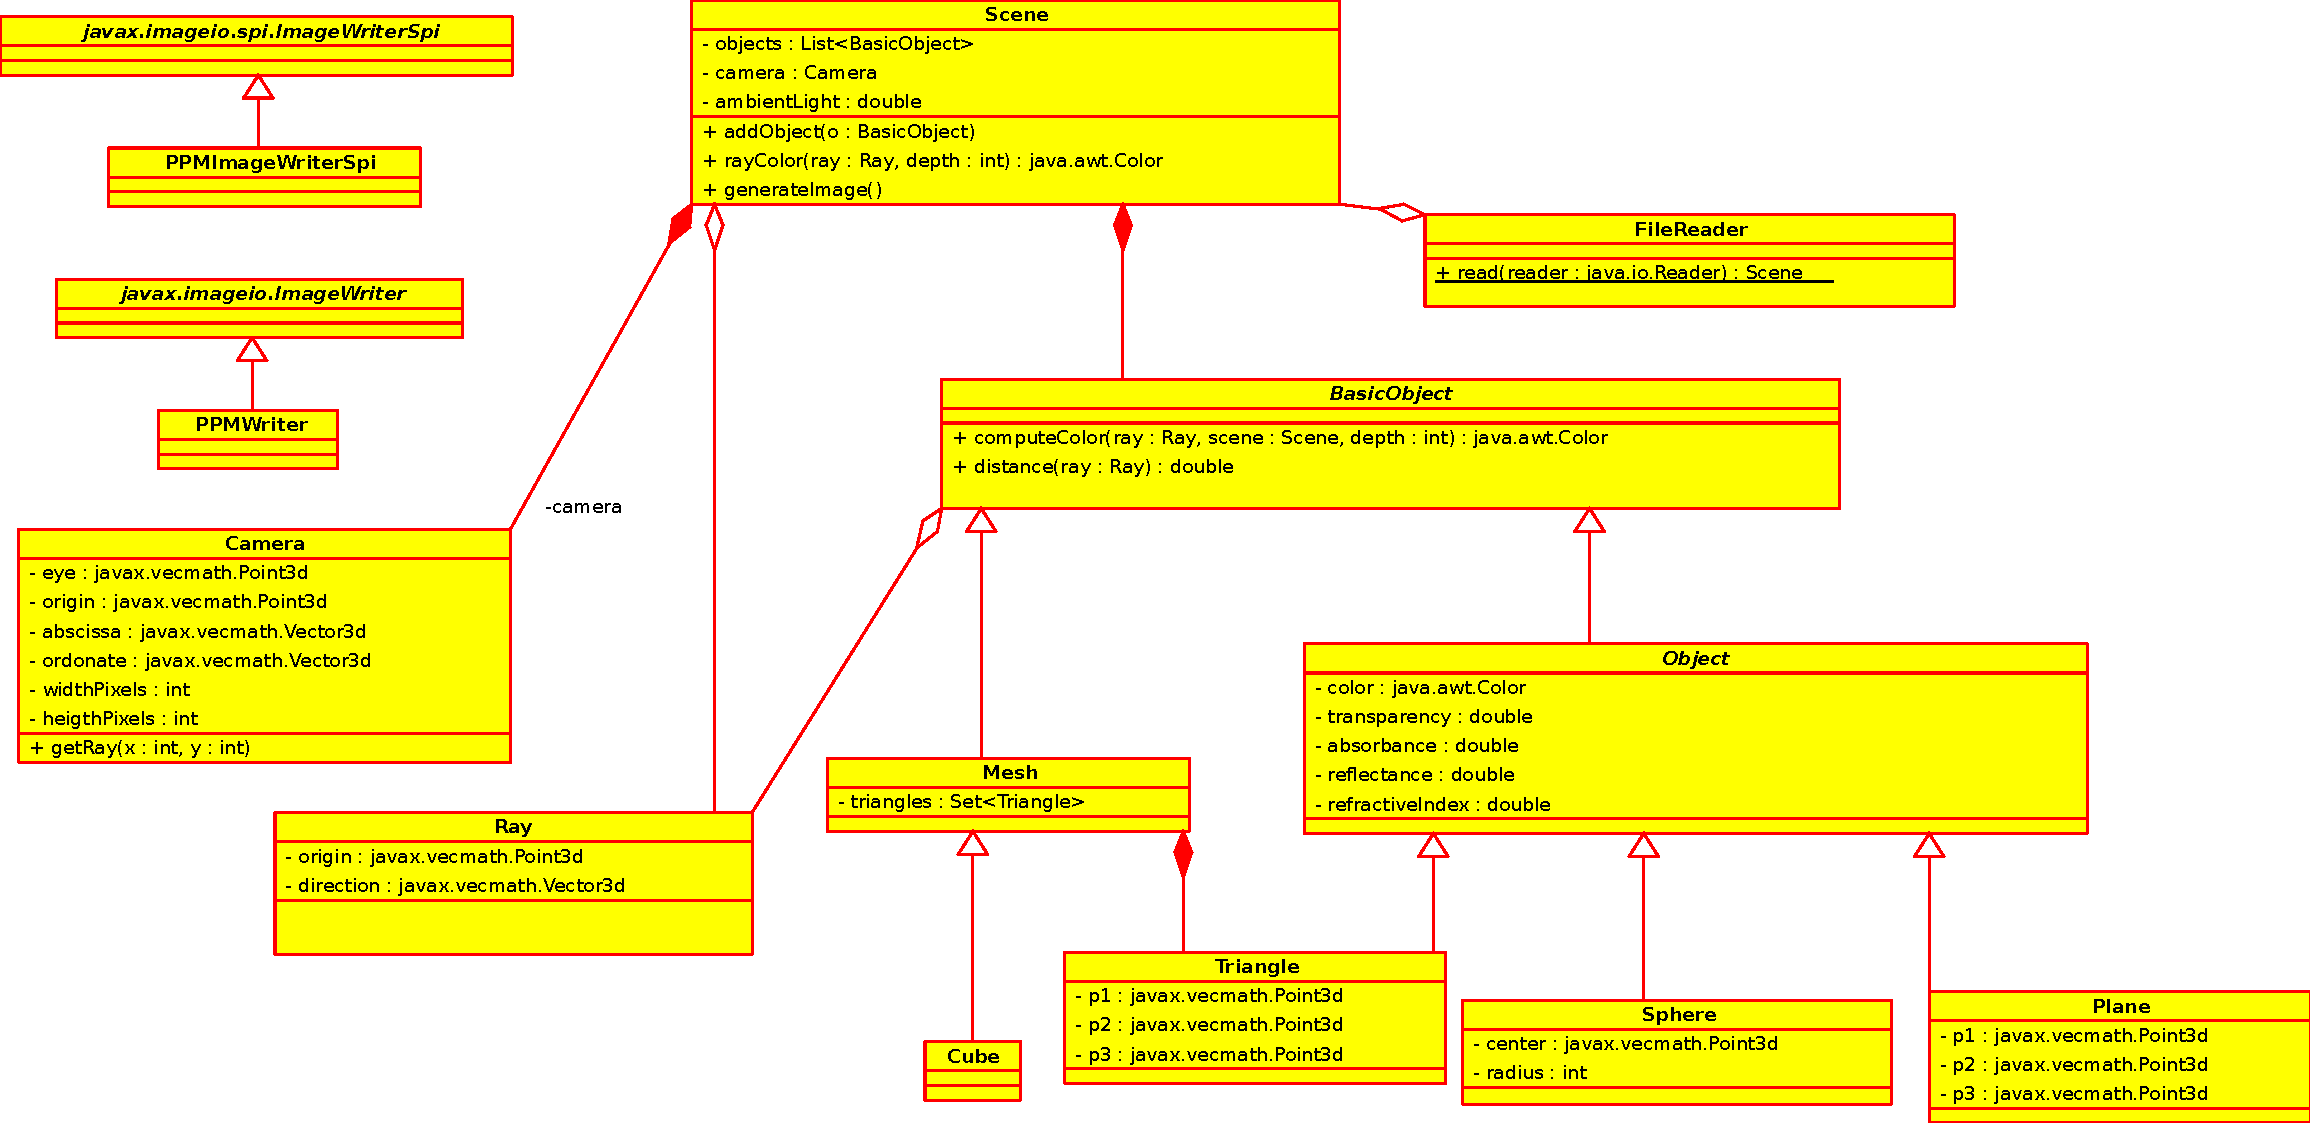
\includegraphics[width=25cm]{uml.pdf}}
          \caption{Diagramme UML\label{fig:uml}}
        \end{figure}
      \end{landscape}
      \restoregeometry
      \clearpage
    }

    Ainsi, l'objet \verb+Scene+ dispose d'une méthode pour calculer la couleur
    d'un rayon passé en paramètre.
    Pour le faire, il va regarder quel objet va intersecter avec le rayon en
    premier, et appeler la méthode \verb+computeColor+ de l'objet en question.

    Cette méthode, définie dans la classe \verb+Object+, va faire tous les
    calculs nécessaires pour calculer les différentes composantes. Pour cela,
    elle peut même appeler à nouveau la méthode \verb+rayColor+ de la classe
    scène, sur les rayons réfléchis ou réfractés.
    Dans ces calculs, elle va appeler la méthode \verb+normal+, qui va donner
    la normale au point d'intersection du rayon avec l'objet, méthode qui sera
    définie dans des sous-classes, en fonction de l'objet.
\end{document}

